\documentclass[../cheatSheetAlgoritmi.tex]{subfiles}
\begin{document}

\subsection{Esercitazione 13 - 13/05/20}
\textbf{Cubi}

Siano dati $n$ cubi. Su ogni faccia del cubo è presente una lettera dell'alfabeto. Ogni cubo può essere descritto da una stringa di $6$ caratteri (e.g. $abcdef$), che rappresenta le 6 facce del cubo. Sia data una parola costituita da $t \leq n$ caratteri. \textbf{Descrivere} un algoritmo che ritorni $true$ se è possibile comporre la parola utilizzando $t$ degli $n$ cubi (scegliendo una faccia per ognuno di essi), $false$ altrimenti. Discutere correttezza e complessità dell'algoritmo risultante.

Il problema sottoposto fa parte delle Reti di Flusso quindi procediamo in questo modo alla \hfill \break risoluzione:
\begin{itemize}
	\item Costruiamo una Rete di Flusso $G = (V, E, s, p, c)$, dove:
	\begin{itemize}
		\item $V$ è l'insieme dei nodi che è rappresentato dagli $n$ cubi, dalle $t$ lettere e da $s$ e $p$ rispettivamente supersorgente e superpozzo
		\item $E$ è l'insieme degli archi della rete di flusso
		\item $s$ è la supersorgente
		\item $p$ è il superpozzo
		\item $c: V \times V \rightarrow \mathbb{R}$  viene definita funzione di capacità e associa ad ogni coppia di nodi un arco con una determinata capacità
	\end{itemize}
	\item definiamo l'insieme degli archi $E$ come segue:
		\begin{itemize}
			\item Aggiungiamo un arco da $s$ $\forall c_{i} \mid 1 \leq i \leq n$ (ad ogni cubo)
			\item $\forall c_{i} \mid 1 \leq i \leq n$ aggiungiamo un arco $\forall t_{j} \mid 1 \leq j \leq t$ (a ogni lettera della parola) - successivamente la funzione di capacità ci dirà che alcuni di questi archi non sono utili
			\item $\forall t_{j} \mid 1 \leq j \leq t$ aggiungiamo un arco a $p$
		\end{itemize}
	\item definiamo la funzione di capacità $c$ come segue:
	\begin{itemize}
		\item Associamo agli archi uscenti da $s$ capacità $6$ in quanto ogni dado può avere al massimo 6 lettere
		\item Associamo agli archi uscenti da ogni dado capacità 0 se tale lettera non corrisponde alla lettera della parola oppure 1 se invece ha un match
		\item Associamo agli archi entranti nel pozzo una capacità pari a 1 
	\end{itemize}
	\item Calcoliamo ora la complessità dell'algoritmo che sappiamo essere pari a $min$(Ford-Fulkerson, Edmonds-Karp) = $min(\mathcal{O}((V + E) \mid f^{*} \mid), \mathcal{O}(VE^{2}))$:
		\begin{itemize}
			\item Il numero di nodi complessivi è dato da $n + t +2$
			\item Il numero di archi complessivi è dato da $n + nt + t$
			\item Il flusso massimo è pari a $t$
			\item Per Ford-Fulkerson il limite superiore dunque è pari a $\mathcal{O}(n \cdot t^{2})$
			\item Per Edmonds-Karp il limite superiore è pari a $\mathcal{O}(n^{2} \cdot t^{3})$
			\item In questo caso la complessità da scegliere è quella data da Ford-Fulkerson
		\end{itemize}
		\item L'algoritmo restituirà infine $true$ come valore se e solo se il flusso massimo $\mid f^{*} \mid = t$ in quanto vorrà dire che si è trovata una combinazione di dadi per cui è possibile costruire la parola.
\end{itemize}
\begin{figure}[H]
\caption{Rete di Flusso - Cubi}
\centering
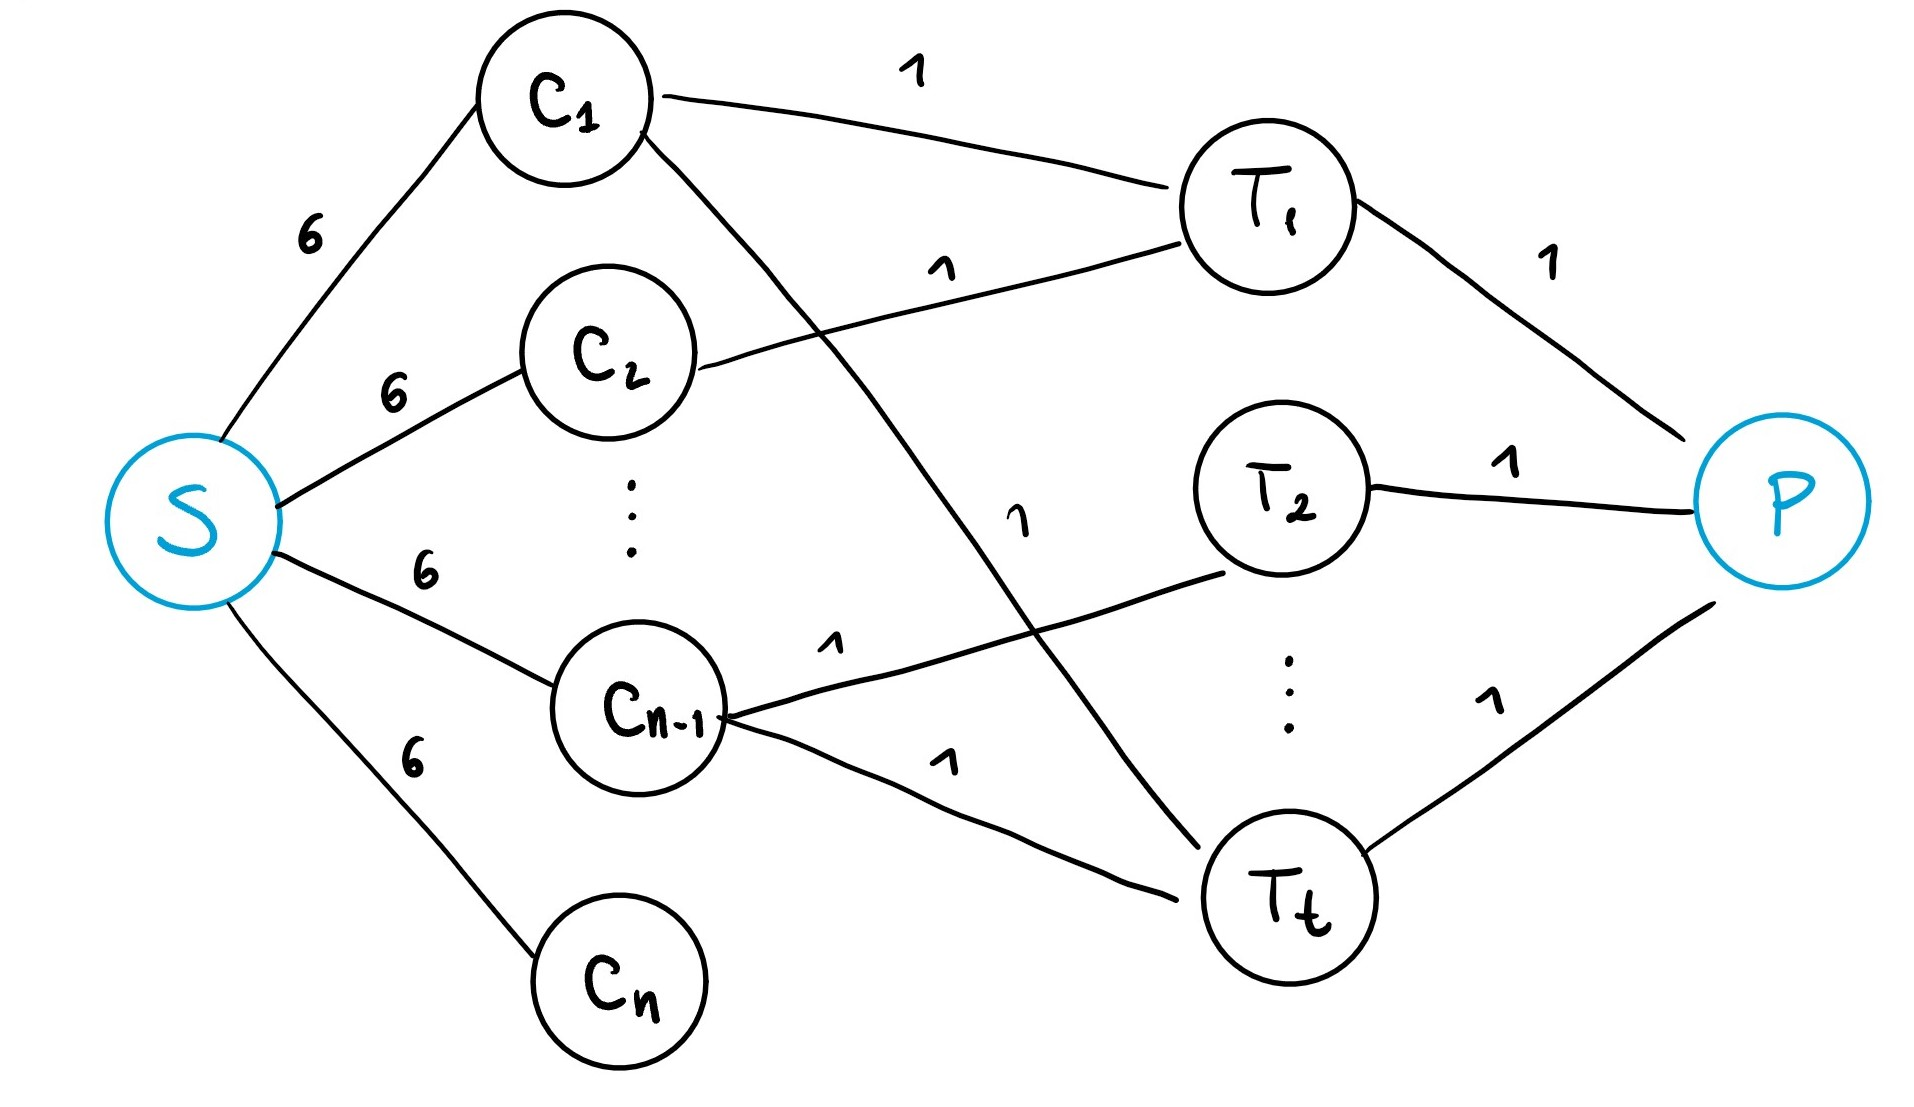
\includegraphics[width=0.5\textwidth]{../img/Locale_2.jpg}
\end{figure}
\textbf{Il gioco delle coppie (2-partition)}\\
Scrivere un algoritmo che, dato un vettore $A$ di $n$ interi distinti ($n$ pari), ritorna $true$ se è possibile partizionare $A$ in coppie di elementi che hanno tutte la stessa somma (intesa come la somma degli elementi della coppia), $false$ altrimenti.\\
Ad esempio: 7,4,5,2,3,6 può essere partizionato in 7 + 2 = 4 + 5 = 3 + 6.\\
Discutere la complessità e la correttezza – per questo esercizio, la dimostrazione di correttezza è importante e va scritta bene.\\
\textbf{Soluzione:} Si può risolvere il problema per step pensando inizialmente al fatto che se è possibile accoppiare gli elementi tra di loro in modo da restituire lo stesso numero se sommati assieme, allora vuol dire che la somma di tutti deve restituire necessariamente un numero intero se divisi per $n / 2$. Il secondo passo per risolverlo è accorgersi che per for sì che tutte le coppie diano come risultato $k$, il numero più grande appartenente all'insieme deve essere abbinato con il numero più piccolo: proviamo a dimostrarlo.
\begin{itemize}
	\item Sia $g \in A$ il numero più grande appartenente all'insieme, $s \in A$ il numero più piccolo e $k$ il numero che risulta dalla somma di ogni coppia
	\item Consideriamo ora anche $g' \in A - \{g\}$ e $s' \in A - \{s\}$ che corrispondono al secondo numero più grande e al secondo numero più piccolo
	\item Assumiamo ora dunque per assurdo che $k = g + s' = g' + s$
	\item Visto che i numeri appartenenti all'insieme sono tutti distinti vuol dire che $g > g'$ e che $s' > s$ e di conseguenza abbiamo che $g + s' > g' + s$, ma ciò contraddice la nostra ipotesi che $k = g + s' = g' + s$
	\item Abbiamo dunque dimostrato che $k = g + s = g' + s'$ 
\end{itemize}
\begin{lstlisting}[caption=2-partition (Coppie)]
bool coppie(int[] A, int n)
	% Ordino i numeri in modo crescente
	mergeSort(A, n)
	int k = A[1] + A[n]
	for i = 2 to n/2 do
		if A[i] + A[n - i + 1] $\neq$ k then
			return false
	return true
\end{lstlisting}
La complessità dell'algoritmo proposto è dunque $\mathcal{O}(n \log n)$ in quanto si utilizza un ordinamento basato su confronti.

\textbf{Stringhe Primitive}

Scrivere un algoritmo che, dati un insieme S contenente $m$ stringhe dette primitive ed una stringa $X[1. . . n]$, conti in quanti modi diversi $X$ è ottenibile dalla concatenazione di stringhe primitive. 

\bigskip

Ad esempio, dato $S=\{01,10,011,101\}$:
\begin{itemize}
	\item $X = 0111010101: $ ci sono 3 modi
(011-10-10-101, 011-10-101-01 e 011-101-01-01)
	\item $X = 0110001:$ non c’è modo di ottenere tre $0$ consecutivi
\end{itemize}
Per comodità, supponete che la lunghezza di una stringa $s$ sia $\mid s \mid$ e di avere a disposizione una primitiva $check(X, s, i)$ che ritorna vero se la stringa $s$ è contenuta nella stringa $X$ a partire dalla posizione $i$. Il costo della chiamata a $check()$ è $\mathcal{O}(\mid s \mid)$. Ad esempio, se $X=1001$ e $s=00$, $check(X, s,2)$ ritorna vero, per tutti gli altri indici $i$ ritorna falso.
\begin{lstlisting}[caption=Stringhe primitive]
int stringhePrimitiveDP(ITEM[] S, ITEM[] X, int m, int n)
	int[] DP = new int[0..n]
	DP[0] = 1
	for i = 1 to n do
		DP[i] = 0
		for j = 1 to m do
			int len = $\mid $S[j]$\mid$
			if i - len $\geq$ 0 and check(X, S[j], i - len) then
				DP[i] = DP[i] + DP[i-len]
	return DP[n]


int stringhePrimitive(ITEM[] S, ITEM[] X, int m, int n)
	int[] DP = new int[1..n]
	for i = 1 to n do
		DP[i] = -1
	return stringhePrimitiveRec(S, X, m, n)

int stringhePrimitiveRec(ITEM[] S, ITEM[] X, int[] DP, int m, int i)
	if i $==$ 0 then
		return 1
	else
		if DP[i] < 0 
			DP[i] = 0
			for j = 1 to m do
			int len = $\mid$S[j]$\mid$
				if  i - len $\geq$ 0 and check(X, S[j], i - len) then
					DP[i] = DP[i] + stringhePrimitiveRec(S, X, DP, m, i - len)
		return DP[i]		
\end{lstlisting}
La soluzione proposta, in entrambe le versioni, programmazione dinamica e memoization, ha complessità computazionale pari a $\mathcal{O}(Snm)$ dovuta al fatto che per riempire ogni cella della tabella delle soluzioni di lunghezza $n$ è necessaria una complessità di $\mathcal{O}(Sm)$. \\
La ricorsione su cui fanno riferimento è la seguente: \\
Sia DP[i] il numero di modi in cui è possibile ottenere il prefisso X[i], allora possiamo definire: 
\begin{equation*}
  	DP[i] =\begin{cases}
        1 & \text{$i = 0$} \\ 
        \sum_{s \in S \land check(X, s, i - \mid s\mid)} DP[i - \mid s \mid] & \text{altrimenti}
  	\end{cases}
\end{equation*}
I casi previsti sono i seguenti:
\begin{itemize}
	\item Se non ho alcun carattere da utilizzare per il confronto con gli elementi di $S$ allora significa che ho completato correttamente la stringa $X$, dunque il valore ritornato è 1
	\item Se invece non è vuota, provo a completare tale stringa sottraendo le stringhe se rispettano il \emph{check()}. Se infatti X(i - S[j], i) combacia con una stringa S[j] dell'insieme S, allora è possibile ridurre il problema ai modi possibili per formare la stringa X(i - S[j], i), questo va fatto per tutte le stringhe che possono che combaciano con il suffisso di X(i). Il valore DP[i] è infatti la somma di tali sotto-problemi. 
	\item Il valore della soluzione è locato in DP[n]
\end{itemize}
\textbf{Sottostruttura ottima} 

Sia $Y = \{\{i\}, ... \{k\}\}$ l'insieme contenente gli insiemi formati dagli indici del vettore $S$ che costituiscono tutti i modi possibili per rappresentare la stringa $X$. 

Supponiamo di considerare la stringa $X - {S[j]}$, ottenuta dalla stringa $X$ rimuovendo la stringa $S[j]$ dal suffisso di $X$, dove $S[j]$ è una stringa dell'insieme $S$; la soluzione ottima per il problema $X - {S[j]}$ sarà costituita dunque da $Y - \{j\}$. Se così non fosse, dovrebbe esistere un insieme $Y' = \{\{i'\}, ... \{k'\}\}$ la cui cardinalità sia superiore a quella di $Y$, ovvero $\mid Y' \mid > \mid Y - \{j\} \mid$. Ma questo è impossibile in quanto $\mid Y' \cup \{j\} \mid > \mid Y \mid$ il che renderebbe $Y' \cup \{j\}$ la soluzione ottima per $X$ violando l'assunzione che vede $Y$ soluzione ottimale per $X$.

\bigskip

\textbf{MC Donald}

Gestire un McDonald non è semplice:
\begin{enumerate}
	\item La giornata lavorativa è suddivisa in 3 turni da 4 ore, dalle 11 alle 23.
	\item Durante il turno $t_{i} \in T$ (dove $T$ l'insieme di 21 turni), è necessario che siano presenti $p_{i}$ unità di personale. 
	\item Avete a disposizione un insieme $D$ di dipendenti; ogni dipendente $d_{j} \in D$ dichiara un insieme di turni $n_{j} \subseteq T$ in cui non può lavorare.
	\item Ad esempio, $d_{j}$ non può lavorare nei turni $\{t_{1}, t_{7}, t_{21}\}$.
	\item Per contratto aziendale, ogni lavoratore non può lavorare per più di 5 turni.
	\item Ogni giorno, un dipendente non può lavorare per più di due turni (qualsiasi, anche non consecutivi).
\end{enumerate}
\textbf{Progettare} un algoritmo che produca uno scheduling che illustri, per ogni turno, il personale associato e discuterne la complessità.\\
\textbf{Soluzione:} Il seguente problema può essere risolto mediante la costruzione di una Rete di Flusso $G = (V, E, s, p, c)$
\begin{itemize}
	\item $V$ è l'insieme dei nodi appartenenti alla rete di flusso ed è costruito come segue 
	\begin{itemize}
		\item Aggiungiamo $D$ nodi, uno per ogni impiegato
		\item Aggiungiamo $7D$ nodi per i giorni lavorativi per ogni impiegato
		\item Aggiungiamo $21$ nodi, cioè pari al numero di $t_{i} \in T$
		\item Aggiungiamo $s$ e $p$ supersorgente e superpozzo 
		\item In totale abbiamo $D + 7D + 21 + 2$ nodi
	\end{itemize}
	\item $E$ è l'insieme degli archi della rete di flusso ed è costruito in questo modo
	\begin{itemize}
		\item Aggiungiamo un arco da $s$ a ogni $D$
		\item Aggiungiamo un arco $\forall d_{i} \mid 1 \leq i \leq D$ a $g_{ij}$ ($ \forall j \mid 1\leq j \leq 7$), cioè da ogni dipendente ai suoi giorni lavorativi
		\item Aggiungiamo un arco $\forall  g_{ij} \mid 1 \leq i \leq D \land 1 \leq i \leq 7$ a $t_{k}$ ($\forall k \mid j+1 \leq k \leq j+3$)
		\item Aggiungiamo infine un arco $\forall t_{k} \mid 1 \leq i \leq T$ entrante in $p$
	\end{itemize}
	\item $s$ è definito supersorgente
	\item $p$ è definito superpozzo
	\item $c: V \times V \rightarrow \mathbb{R}$ è chiamata capacità ed è definita come segue
	\begin{itemize}
		\item Associamo agli archi uscenti da $s$ una capacità pari a 5, in modo che venga rispettato il vincolo 5
		\item Associamo agli archi uscenti da $d_{i}$ ($1 \leq i \leq D$) capacità pari a 2, in modo che venga rispettato il vincolo 6
		\item Associamo agli archi uscenti da $g_{ij}$ ($1 \leq i \leq D$ $\land$ $1 \leq j \leq 7$) capacità 0 nel caso in cui il turno rientra nell'insieme $n_{i}$ dell'impiegato $d_{i}$ altrimenti 1 per rispettare il vincolo 3
		\item Associamo agli archi uscenti da ogni $t_{i}$ ($1 \leq i \leq T$) una capacità pari a $p_{i}$, in modo da rispettare il vincolo 2
	\end{itemize}
	\item La complessità dell'algoritmo proposto è pari a \hfill \break $min$(Ford-Fulkerson, Edmonds-Karp) = $min(\mathcal{O}((V + E) \mid f^{*} \mid), \mathcal{O}(VE^{2}))$:
		\begin{itemize}
			\item Il numero di nodi complessivi è dato da $D + 7D + 21 + 2 = 8D + 23$
			\item Il numero di archi complessivi è dato da $D + 7D + 21D + 21 = 29D + 21$
			\item Il flusso massimo è pari a $5D$ oppure a $\sum_{i = 1}^{21}p_{i}$ (unità di personale legata al turno $i$-esimo)
			\item Per Ford-Fulkerson il limite superiore dunque è pari a $\mathcal{O}(D^{2})$
			\item Per Edmons-Karp il limite superiore è pari a $\mathcal{O}(D^{3})$
			\item In questo caso la complessità da scegliere è quella data da Ford-Fulkerson
		\end{itemize}
\end{itemize}
\begin{figure}[H]
\caption{Rete di Flusso - MC Donald}
\centering
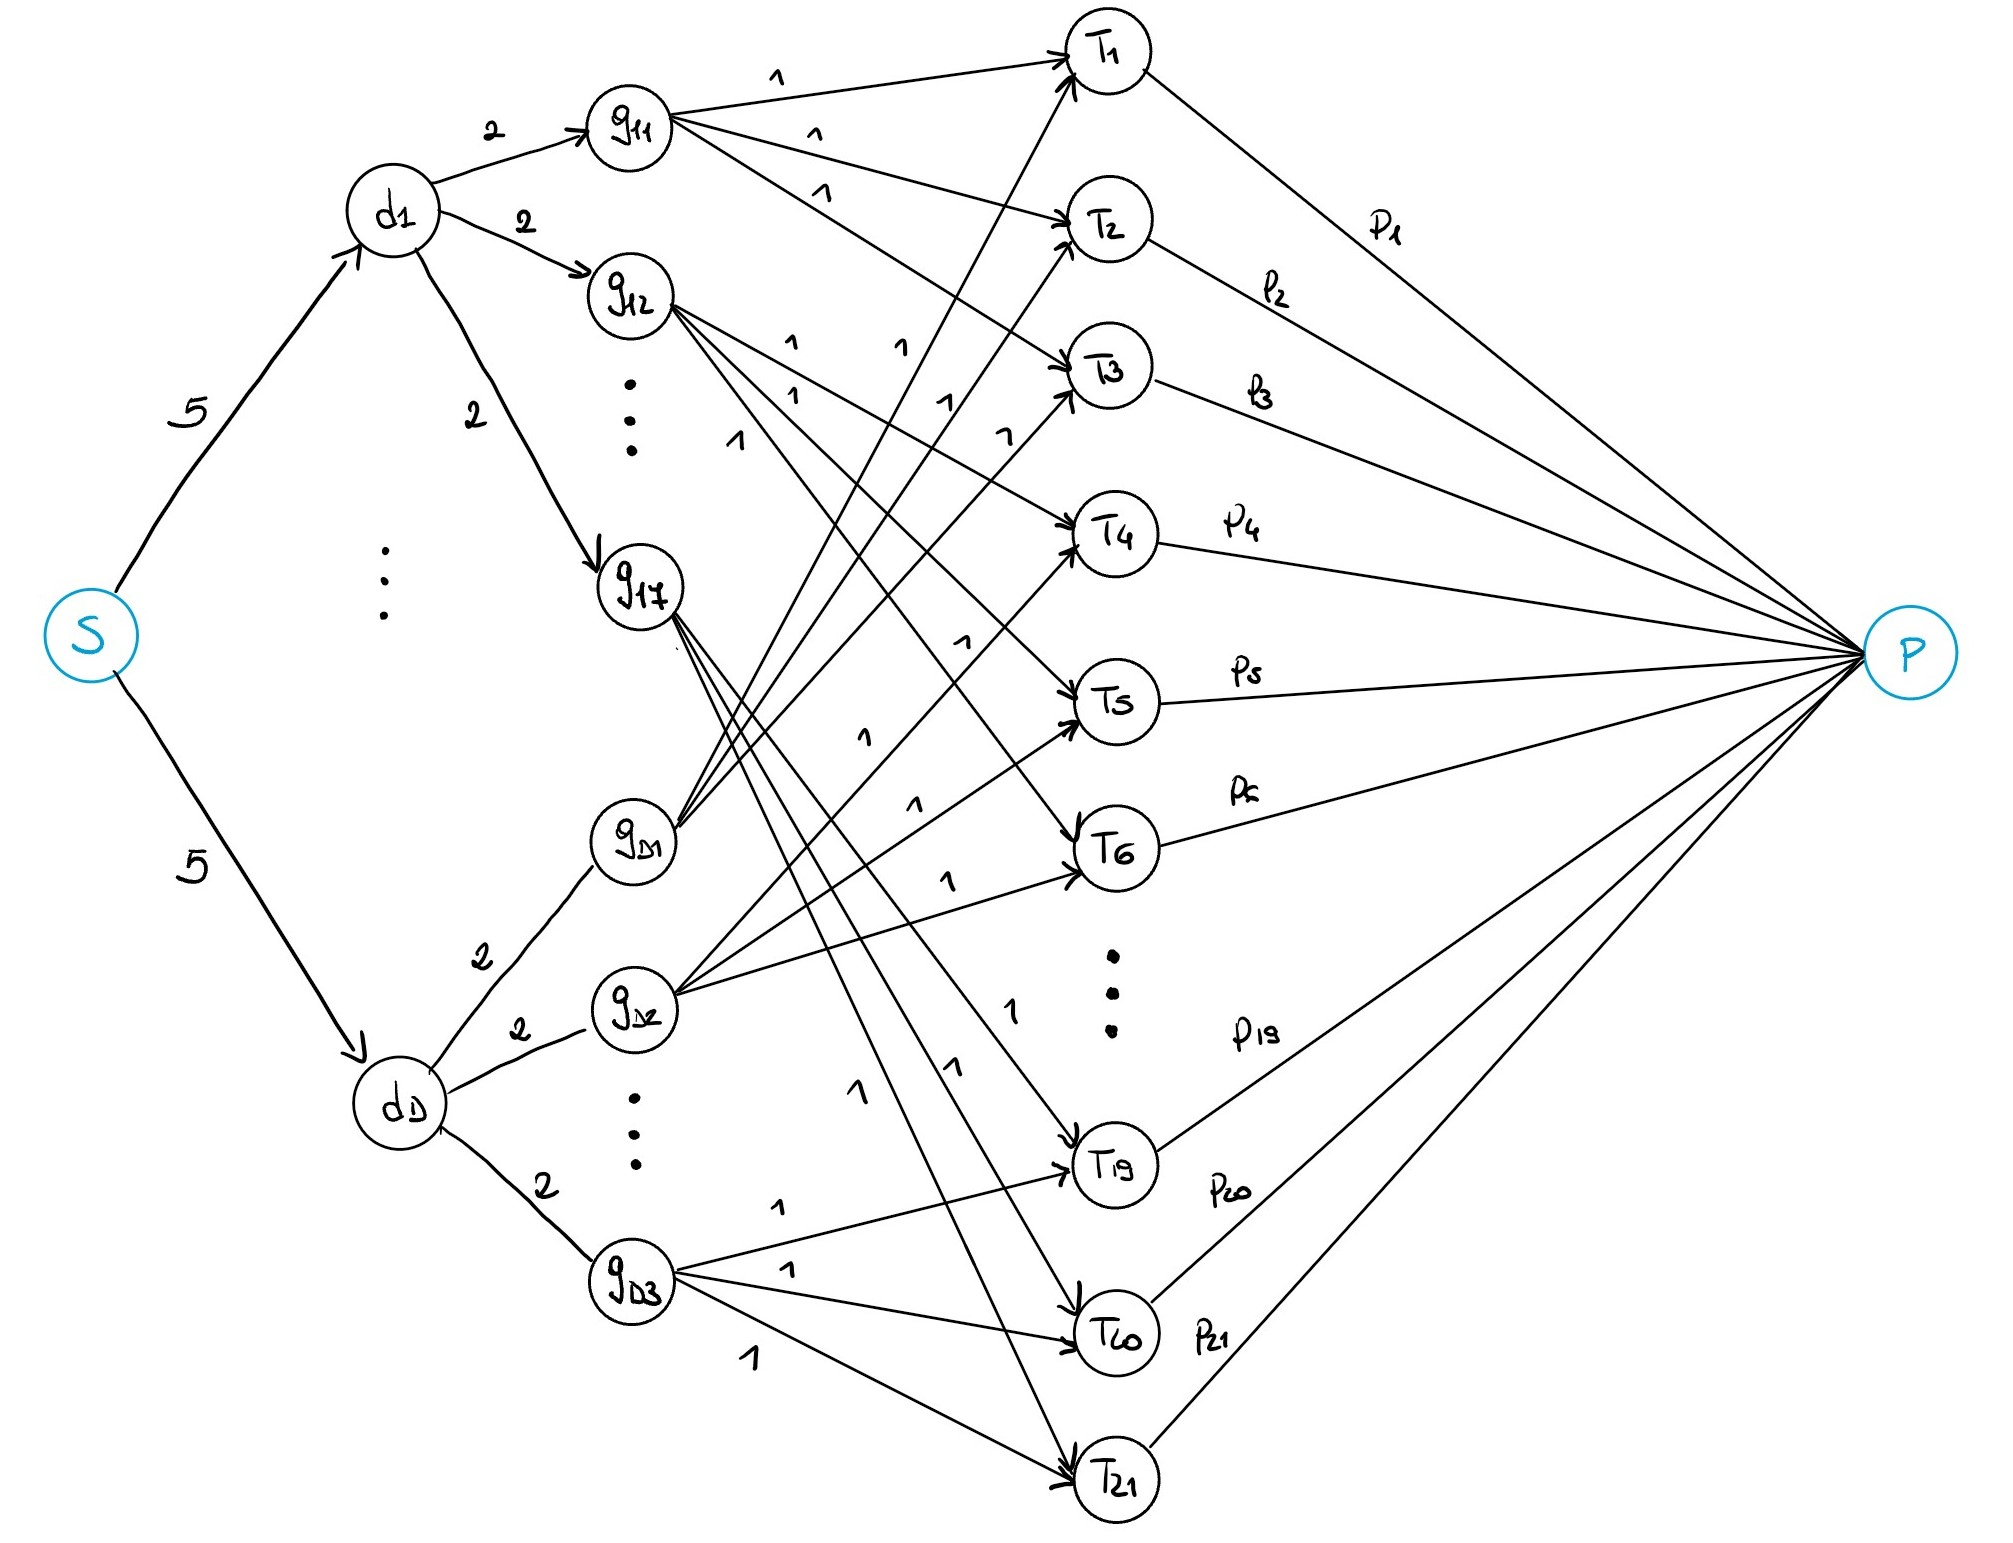
\includegraphics[width=0.5\textwidth]{../img/Locale_3.jpg}
\end{figure}
\textbf{Anagrammi}

Un'anagramma è una parola o frase ottenuta riarrangiando le lettere di un'altra parola o frase. Per esempio, "notremors" è un anagramma di "montresor". Si supponga di avere in input un vettore di $n$ stringhe di lunghezza massima $k$; si scriva un algoritmo che stampi in output tutti i gruppi di anagrammi contenuti in queste $n$ stringhe. Se ne discuta correttezza e complessità.

Esempio di input: rosa, pippo, poppi, raso, orsa, giappone

Esempio di output: \{rosa, raso, orsa\}, \{pippo, poppi\}, \{giappone\}

\begin{lstlisting}[caption=anagrammi]
anagrams(ITEM[] S, int n)
	HASH H $\leftarrow$ Hash()
	for i = 1 to n do
		% Riordiniamo le lettere che compongono una parola
		sorted $\leftarrow$ sort(S[i])
		% Controlliamo se la parola ordinata era gia' presente
		SET S $\leftarrow$ H.lookup(sorted)
		if S = nil then
			% Se non era presente creiamo il suo set
			S $\leftarrow$ Set()
		% La inseriamo nell'insieme degli anagrammi di quelle lettere
		S.insert(S[i])
		% E reinseriamo il tutto con la chiave delle lettere ordinate
		H.insert(sorted, S)
	foreach x $\in$ H do
		SET S $\leftarrow$ H.lookup(x)
		print S
\end{lstlisting}
Visto che un anagramma non è altro che una permutazione di un insieme di lettere è possibile capire o meno se una sequenza di lettere è un anagramma di un'altra sequenza semplicemente riordinandole. Il costo dell'ordinamento è pari a $\mathcal{O}(k \log{k}$) visto che le stringhe sono lunghe al massimo $k$ e il controllo di tutte le stringhe richiede tempo lineare $\mathcal{O}(n)$ come anche la stampa. L'inserimento all'interno della struttura, la lookup e l'inserimento set richiedono tempo $\mathcal{O}(1)$.

Il costo complessivo dell'algoritmo è quindi pari a $\mathcal{O}(nk \log{k})$.

In alternativa a questa soluzione è anche possibile immaginare di utilizzare un singolo set al cui interno vengono inserite le varie lettere che compongono una parola e controllare le altre, man mano rimuovendole dall'insieme nel caso in cui siano permutazione stampandole. Il costo di questa soluzione è pari a $\mathcal{O}(k \cdot n^{2})$ supponendo che l'operazione contains costi $\mathcal{O}(1)$.
\newpage
\end{document}